\chapter{Ajouter une page au site}

\section{Création du Front-End}
Afin d'inclure de nouvelles fonctionnalités, il est possible d'ajouter de nouvelles pages au site. Pour ce faire, il faut dans un premier temps créer un fichier HTML et le placer dans le dossier \textit{ASMAE/tennis/templates}. Il est intéressant de noter que les différents éléments statiques (style, polices, images ou scripts) doivent être ajoutés dans les dossiers correspondants (css, fonts, img, js)  présents dans le répertoire \textit{ASMAE/tennis/static/tennis}.\\

%A changer

%Une fois , il est nécessaire de créer une view dans le fichier views.py se trouvant dans le dossier "ASMAE/tennis", qui reprendra la page à renvoyer quand un utilisateur fera une requête pour obtenir la page. Le format le plus classique et simpliste d'une telle requête est le suivant: on définit le nom de la requête, ainsi que la page à rendre quand celle-ci est effectuée.\\

%\begin{figure}[H]
%\centering
%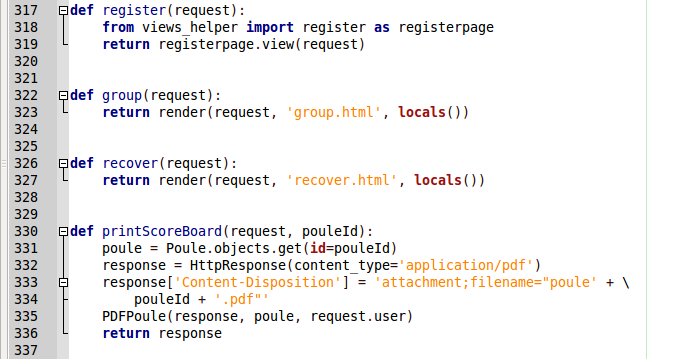
\includegraphics[scale=0.4]{views.png}
%\caption{Fichier views.py}
%\end{figure}

%Enfin, il reste à ajouter au fichier urls.py (également présent dans le dossier "ASMAE/tennis") qui contient tous les liens URL disponibles sur le site, ainsi que le lien vers le nom des views concernées. Pour ce faire, il suffit de rajouter une nouvelle ligne dans le fichier, en respectant le format suivant : url(NouveauLienUrl, NomDeLaViews), .

%\begin{figure}[H]
%\centering
%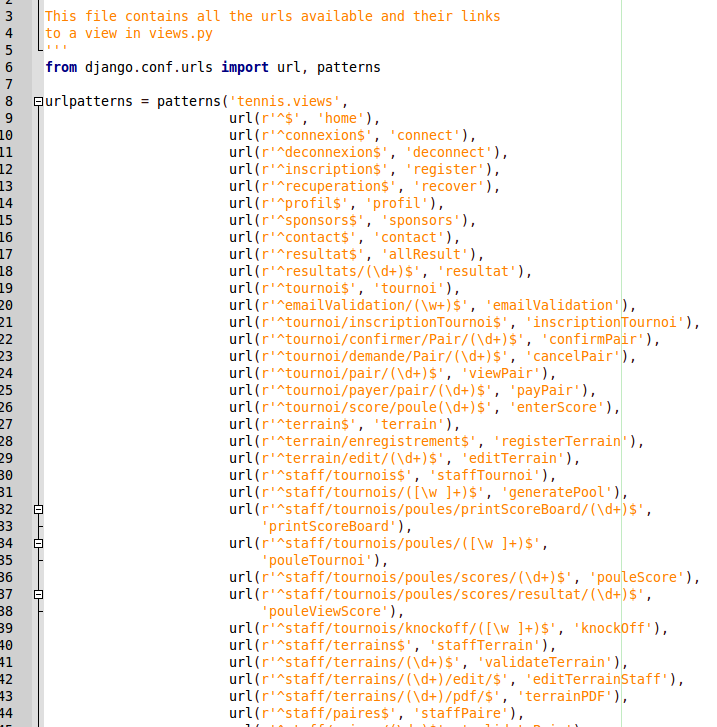
\includegraphics[scale=0.4]{url.png}
%\caption{Fichier urls.py}
%\end{figure}

\section{Gestion du Back-End}

\subsection{Récupération des informations de la base de données vers les pages web}

\subsection{Enregistrer des informations des pages web vers la base de données}